\chapter{Pose estimation II: Relative pose from synthetic data}

We now know that a neural network can extract 2D image coordinates of some
features and use these to infer poses in some other coordinate frame.  This is
however under the assumption that the camera position is constant with respect
to the target coordinate frame. We have also seen that this estimation is
reliable enough to perform the pushing task using the resulting cube pose
estimates. What if we could extract 2D image locations of features but the
camera position is unknown and changing? If some features in the image defines
a coordinate frame that are accessible to us, then an algorithm should
theoretically be able to infer these poses in this coordinate frame as long as
those features are visible. For the following experiment, we assume that we
know the projected 2D locations of some features in 3D space, where the 2D plane
is randomly placed.

\section{Method}
\label{subsec:sim_moving}

Since the region around the end-effector in these experiments is non-symmetric
(see left part of figure \ref{fig:end-effector-frame}), this area could be used
to define a coordinate frame as long as this part is visible to the camera. Let
this coordinate frame be defined as in the right side of figure
\ref{fig:end-effector-frame}.

\begin{figure}[h!]
    \centering
    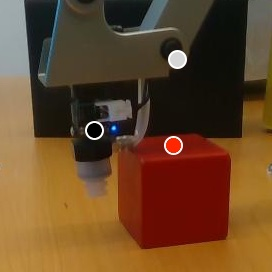
\includegraphics[width=0.32 \textwidth]{res/pose-feature-points.jpg}
    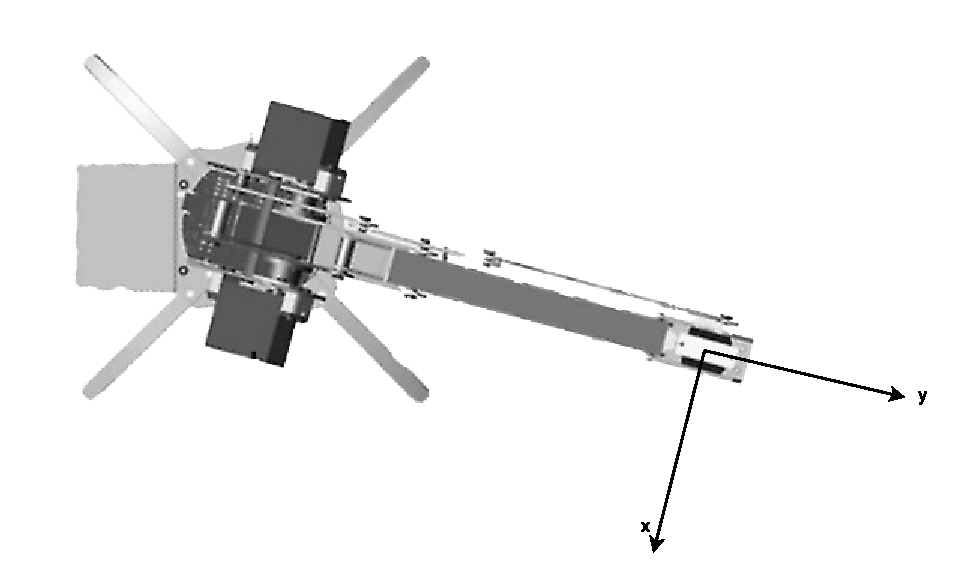
\includegraphics[width=0.5 \textwidth]{res/end-effector-frame.pdf}

    \caption{If the section of the robot to the left is visible, it can define
    a coordinate frame for the cube invariant to camera rotation and
    translation.}

    \label{fig:end-effector-frame}
    
\end{figure}

Inspired by the three marked points in figure \ref{fig:end-effector-frame}, an
environment was setup where these points together with different camera
positions and orientations could be sampled and projected onto a 2D plane (the
image). Some samples are shown in figure \ref{fig:pose-sim-setup}. The target
values were given in the frame of the end effector; a 2D horizontal coordinate
frame with the origin at the suction cup and x-, and y-axes parallel to the
table.

\begin{figure}[h!]
    \centering
    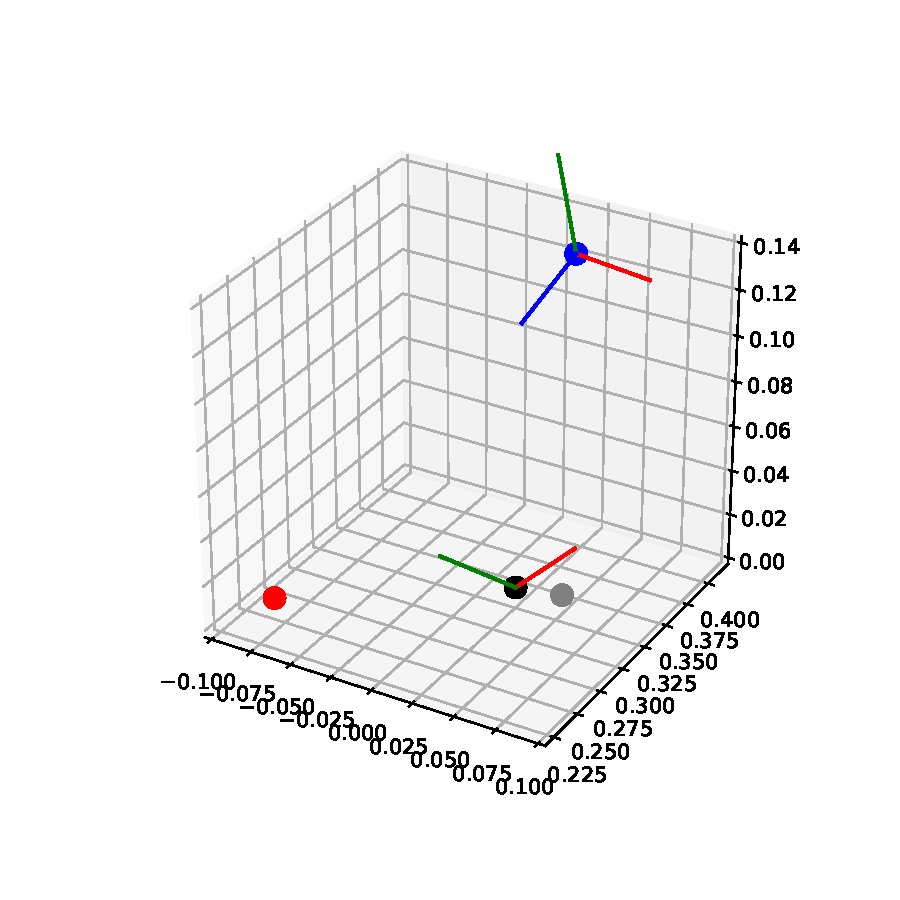
\includegraphics[width=0.32 \textwidth]{res/pose_sim_setup1.pdf}
    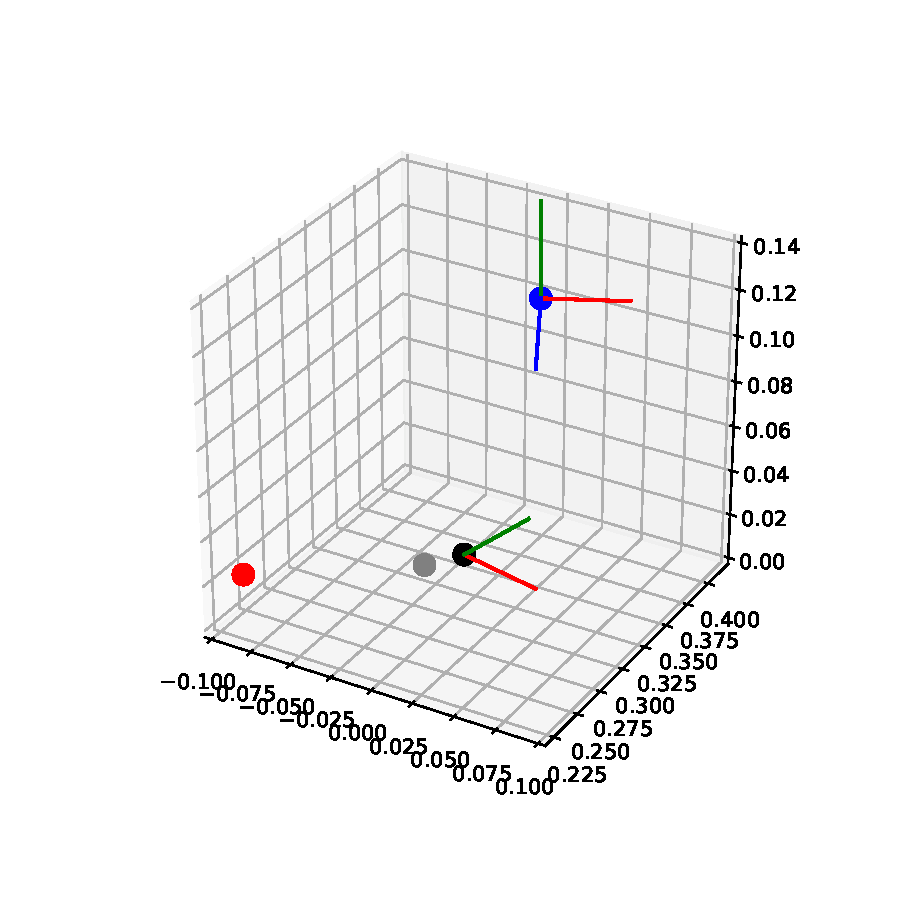
\includegraphics[width=0.32 \textwidth]{res/pose_sim_setup2.pdf}
    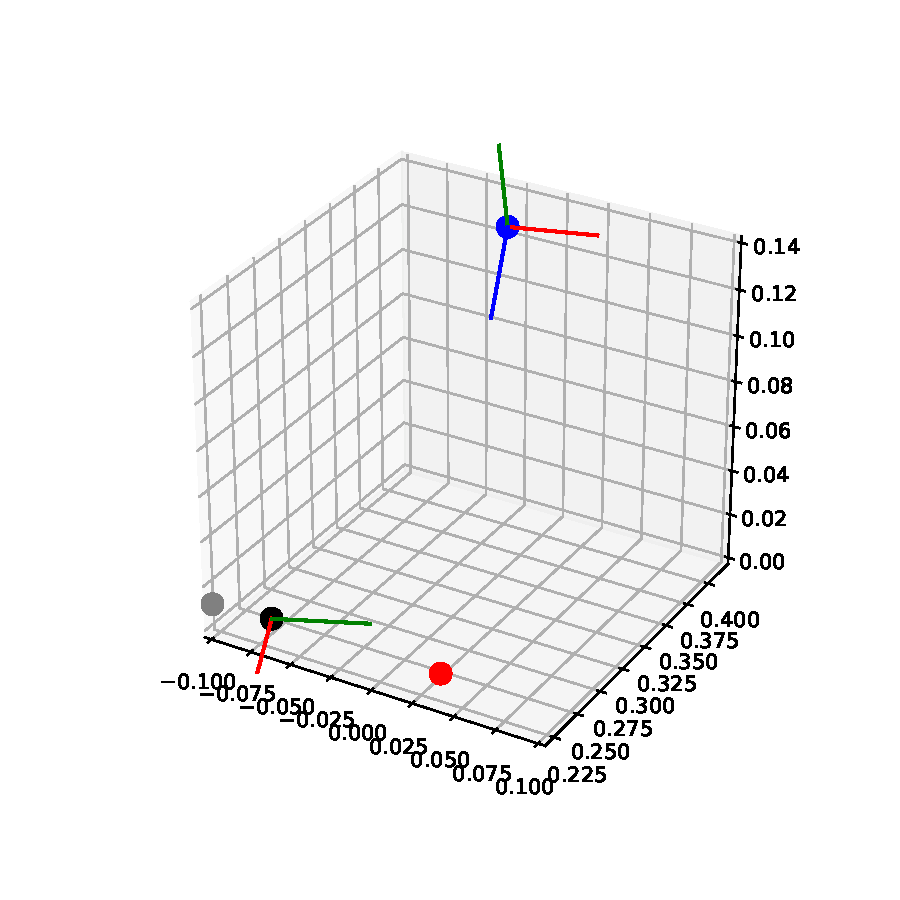
\includegraphics[width=0.32 \textwidth]{res/pose_sim_setup3.pdf}

    \caption{Sampled camera (blue), cube (red), and robot poses (black and
    gray). Target values were cube poses in the frame given by the robot, here
    seen with origin in the black point with x-, and y-axis shown as the red
    and green lines. Input data were the three points projected onto a 2D
    plane given by the camera and a focal length $f$. Comparisons were made
    when appending a third dimension to the picture, which was the length from
    camera to each point.}

    \label{fig:pose-sim-setup}
    
\end{figure}

All the operations needed to infer the target values from known 3D coordinates
were linear transformations, giving rise to question if it is sufficient to
regress a linear model. Experiments were therefore done with a linear model,
and a one and two hidden layer model with 100 hidden ELU-activated units and
batch normalization, and including or excluding depth information. The loss was
mean squared error and the networks were trained using the Adam optimizer.

\section{Results \& Discussion}

As can be seen in figure \ref{fig:pose-sim-losses} and \ref{fig:pose-sim-corr},
deeper networks achieve better results. 2D coordinates were also shown to be
sufficient, although depth information here improves the results.
Interestingly, the predictions for a 2 hidden layer with depth information are
still quite noisy, even though the 2D feature points are readily available and
given without noise. This raises concerns to whether good enough results can be
achieved with real data where feature coordinates are inferred by a
convolutional neural network, and also where labels are produced with noise.

\begin{figure}[h!]
    \centering
    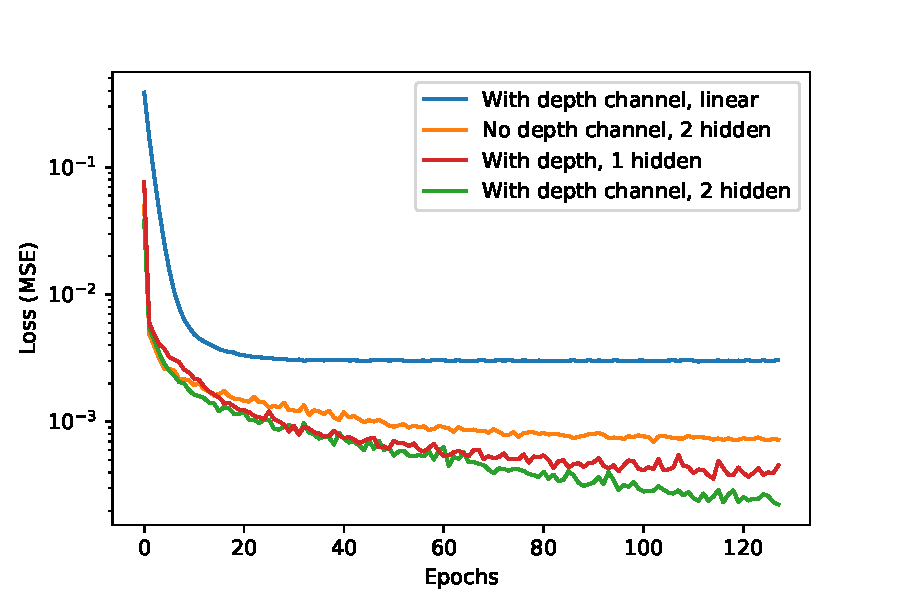
\includegraphics[width=0.7 \textwidth]{res/pose_sim_losses.pdf}

    \caption{Training losses for pose estimation of simulated robot and cube.
    Losses for neural networks given different parametrizations and input
    data.}

    \label{fig:pose-sim-losses}
    
\end{figure}

\begin{figure}[h!]
    \centering
    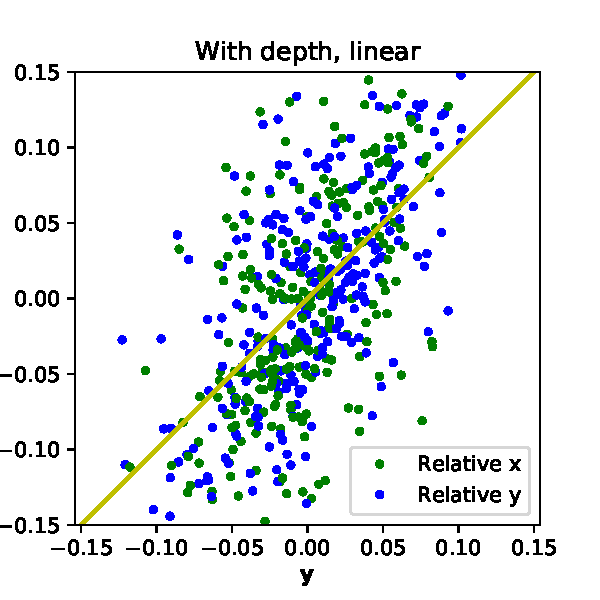
\includegraphics[width=0.49 \textwidth]{res/pose_sim_depth_linear.pdf}
    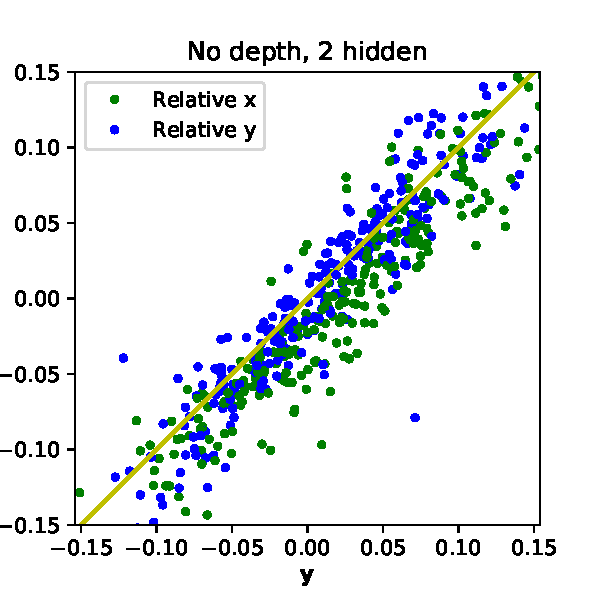
\includegraphics[width=0.49 \textwidth]{res/pose_sim_nodepth_2hidden.pdf}
    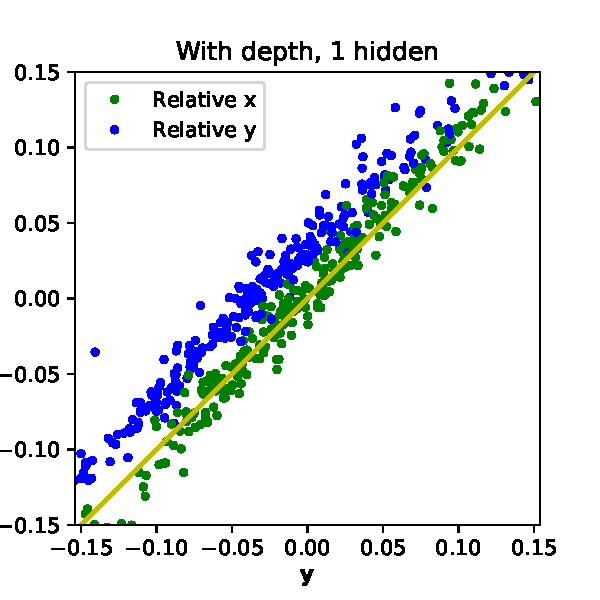
\includegraphics[width=0.49 \textwidth]{res/pose_sim_depth_1hidden.pdf}
    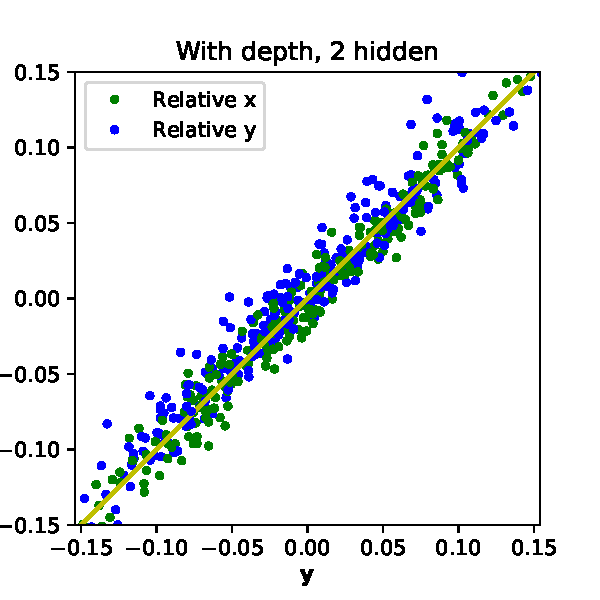
\includegraphics[width=0.49 \textwidth]{res/pose_sim_depth_2hidden.pdf}

    \caption{Pose estimation from a simulated environment and camera. Target
    $x$ (green) and target $y$ (blue) values (horizontal axis) plotted against
    the predicted $x$ and $y$ values (vertical axis).  Plot 1: Depth
    information was provided to the two points on the robot and the cube.
    Network was only a linear layer. Plot 2: Only 2D coordinates were given as
    inputs, network had 2 hidden layers.  Plot 3: Depth was given, network
    using 1 hidden layer.  Plot 4: Depth was given, network using 2 hidden
    layers.}

    \label{fig:pose-sim-corr}
    
\end{figure}
